\documentclass{standalone}
\usepackage{tikz}
\usetikzlibrary{patterns, positioning}
\usepackage[sfdefault]{ClearSans} %% option 'sfdefault' activates Clear Sans as the default text font
\usepackage[T1]{fontenc}

\begin{document}
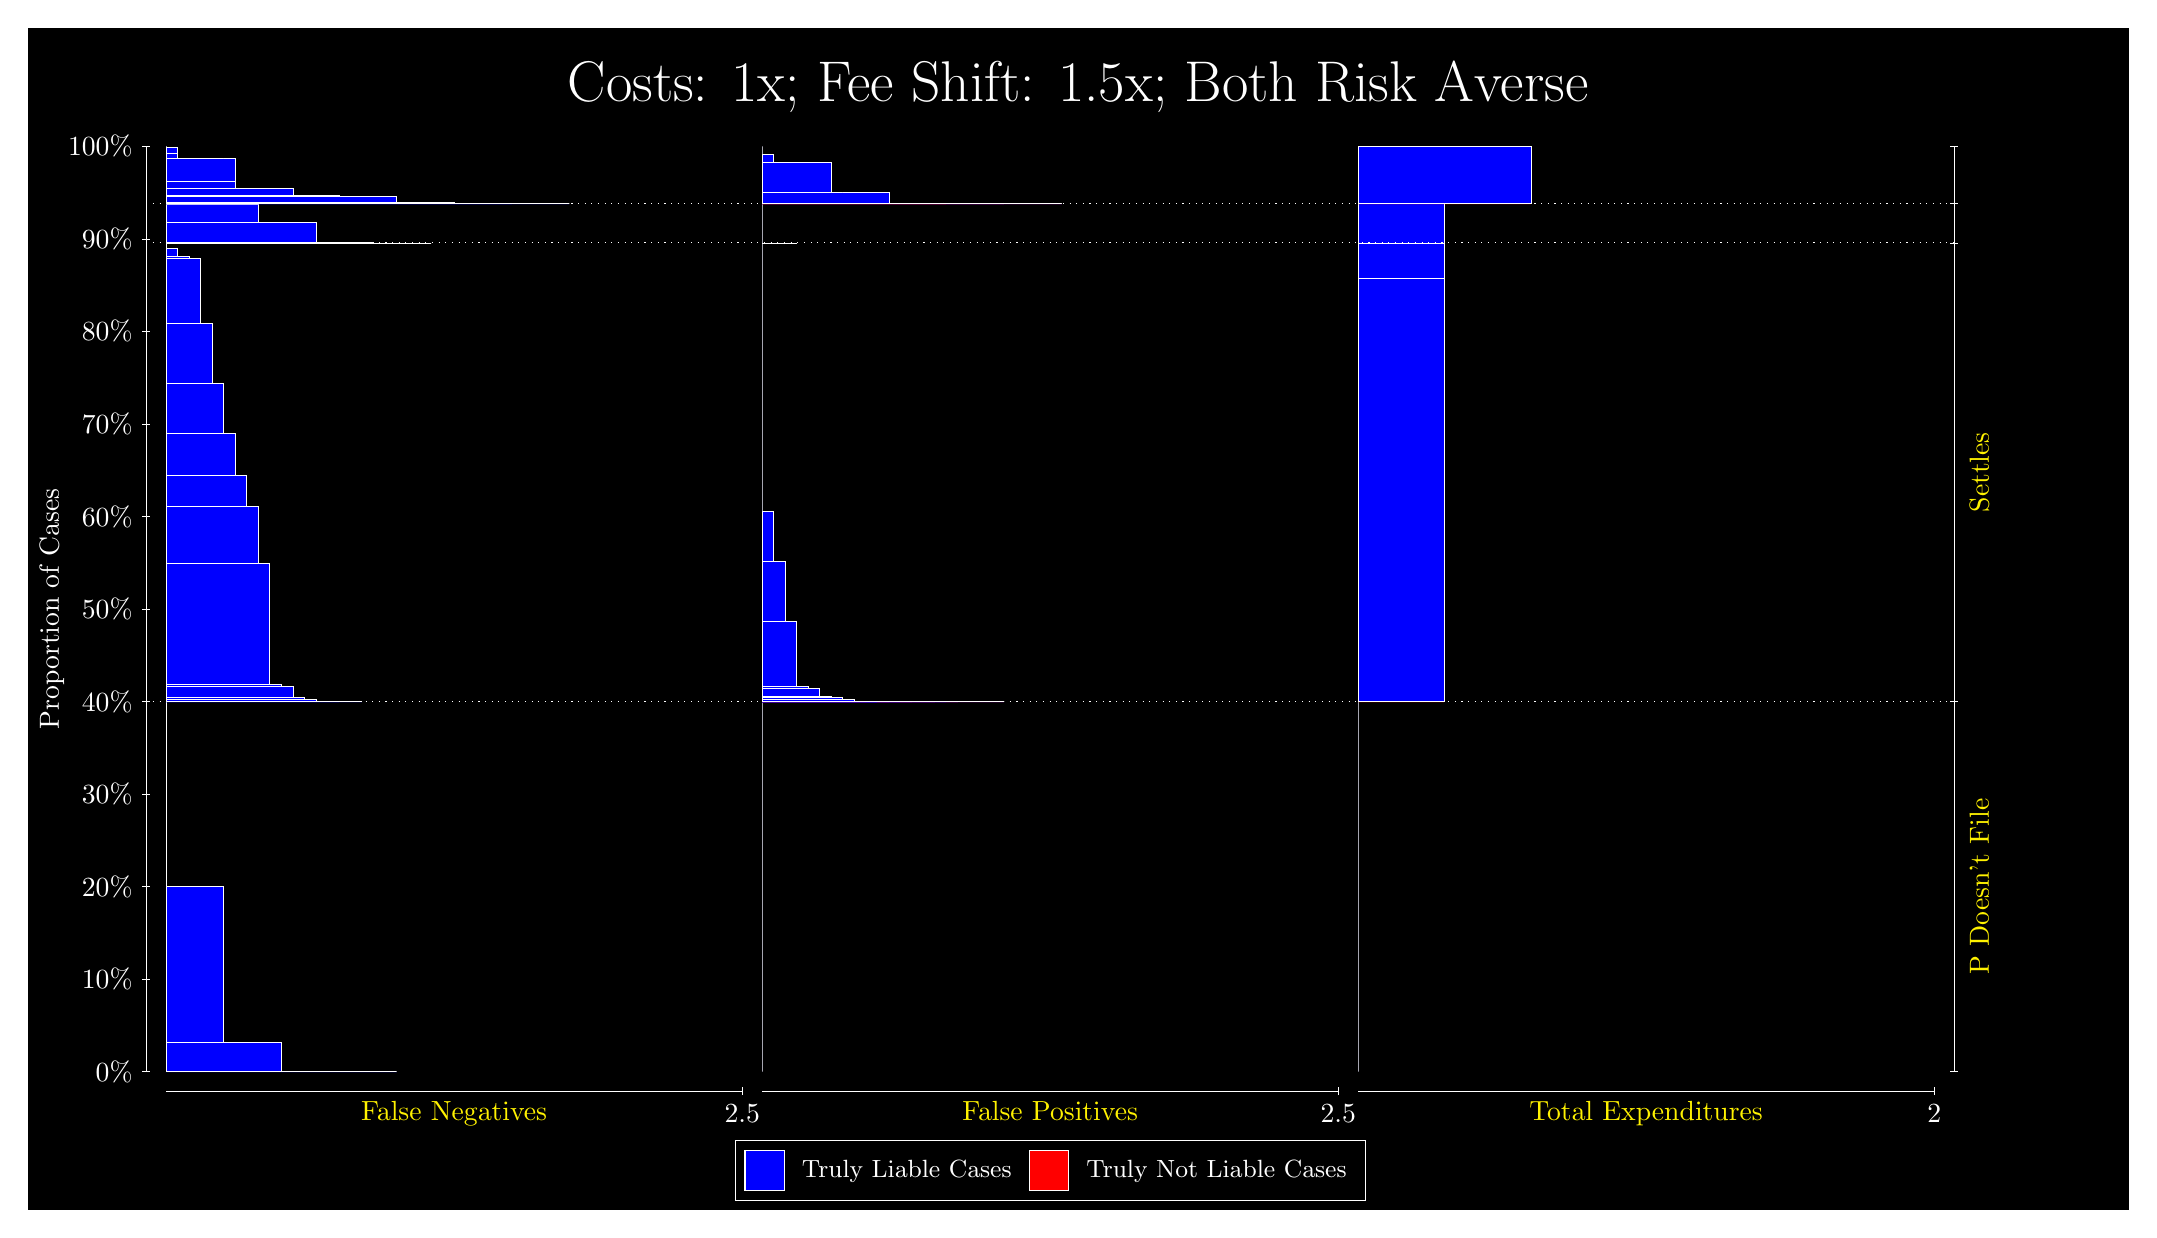
\begin{tikzpicture}
\draw[fill=black] (0,0) rectangle (26.667,15);
\draw[text=white] (0,13.5) rectangle (26.667,15) node[midway] {\huge Costs: 1x; Fee Shift: 1.5x; Both Risk Averse};
\draw[white, very thin] (1.5,1.75) -- (1.5,13.5);
\node[rotate=90, text=white, anchor=center] at (0.3, 7.625) {Proportion of Cases};
\draw[white, very thin] (1.45,1.75) -- (1.55,1.75);
\node[text=white, anchor=east] at (1.45, 1.75) {0\%};
\draw[white, very thin] (1.45,2.925) -- (1.55,2.925);
\node[text=white, anchor=east] at (1.45, 2.925) {10\%};
\draw[white, very thin] (1.45,4.1) -- (1.55,4.1);
\node[text=white, anchor=east] at (1.45, 4.1) {20\%};
\draw[white, very thin] (1.45,5.275) -- (1.55,5.275);
\node[text=white, anchor=east] at (1.45, 5.275) {30\%};
\draw[white, very thin] (1.45,6.45) -- (1.55,6.45);
\node[text=white, anchor=east] at (1.45, 6.45) {40\%};
\draw[white, very thin] (1.45,7.625) -- (1.55,7.625);
\node[text=white, anchor=east] at (1.45, 7.625) {50\%};
\draw[white, very thin] (1.45,8.8) -- (1.55,8.8);
\node[text=white, anchor=east] at (1.45, 8.8) {60\%};
\draw[white, very thin] (1.45,9.975) -- (1.55,9.975);
\node[text=white, anchor=east] at (1.45, 9.975) {70\%};
\draw[white, very thin] (1.45,11.15) -- (1.55,11.15);
\node[text=white, anchor=east] at (1.45, 11.15) {80\%};
\draw[white, very thin] (1.45,12.325) -- (1.55,12.325);
\node[text=white, anchor=east] at (1.45, 12.325) {90\%};
\draw[white, very thin] (1.45,13.5) -- (1.55,13.5);
\node[text=white, anchor=east] at (1.45, 13.5) {100\%};

\draw[white, very thin] (24.457,1.75) -- (24.457,13.5);
\draw[white, very thin] (24.407,1.75) -- (24.507,1.75);
\node[anchor=west] at (24.407, 1.75) {};
\draw[white, very thin] (24.407,6.4489) -- (24.507,6.4489);
\node[anchor=west] at (24.407, 6.4489) {};
\draw[white, very thin] (24.407,12.273) -- (24.507,12.273);
\node[anchor=west] at (24.407, 12.273) {};
\draw[white, very thin] (24.407,12.772) -- (24.507,12.772);
\node[anchor=west] at (24.407, 12.772) {};
\draw[white, very thin] (24.407,13.5) -- (24.507,13.5);
\node[anchor=west] at (24.407, 13.5) {};

\draw[white, very thin, fill=blue] (1.75,1.75) rectangle (4.6775,1.75);
\draw[white, very thin, fill=blue] (1.75,1.75) rectangle (3.9457,1.7532);
\draw[white, very thin, fill=blue] (1.75,1.7532) rectangle (3.2138,2.126);
\draw[white, very thin, fill=blue] (1.75,2.126) rectangle (2.4819,4.1027);
\draw[white, very thin, fill=red] (1.75,4.1027) rectangle (1.75,4.1027);
\draw[white, very thin, fill=blue] (1.75,4.1027) rectangle (1.75,6.4489);
\draw[white, very thin, fill=blue] (1.75,6.4489) rectangle (4.2384,6.4489);
\draw[white, very thin, fill=blue] (1.75,6.4489) rectangle (3.9457,6.449);
\draw[white, very thin, fill=blue] (1.75,6.449) rectangle (3.6529,6.4784);
\draw[white, very thin, fill=blue] (1.75,6.4784) rectangle (3.5065,6.499);
\draw[white, very thin, fill=blue] (1.75,6.499) rectangle (3.3602,6.6464);
\draw[white, very thin, fill=blue] (1.75,6.6464) rectangle (3.2138,6.6659);
\draw[white, very thin, fill=blue] (1.75,6.6659) rectangle (3.0674,8.2009);
\draw[white, very thin, fill=blue] (1.75,8.2009) rectangle (2.921,8.9242);
\draw[white, very thin, fill=blue] (1.75,8.9242) rectangle (2.7746,9.3207);
\draw[white, very thin, fill=blue] (1.75,9.3207) rectangle (2.6283,9.8609);
\draw[white, very thin, fill=blue] (1.75,9.8609) rectangle (2.4819,10.491);
\draw[white, very thin, fill=blue] (1.75,10.491) rectangle (2.3355,11.25);
\draw[white, very thin, fill=blue] (1.75,11.25) rectangle (2.1891,12.079);
\draw[white, very thin, fill=blue] (1.75,12.079) rectangle (2.0428,12.109);
\draw[white, very thin, fill=blue] (1.75,12.109) rectangle (1.8964,12.2);
\draw[white, very thin, fill=red] (1.75,12.2) rectangle (1.75,12.2);
\draw[white, very thin, fill=blue] (1.75,12.2) rectangle (1.75,12.273);
\draw[white, very thin, fill=blue] (1.75,12.273) rectangle (5.1167,12.273);
\draw[white, very thin, fill=blue] (1.75,12.273) rectangle (4.3848,12.277);
\draw[white, very thin, fill=blue] (1.75,12.277) rectangle (3.6529,12.541);
\draw[white, very thin, fill=blue] (1.75,12.541) rectangle (2.921,12.769);
\draw[white, very thin, fill=blue] (1.75,12.769) rectangle (2.1891,12.772);
\draw[white, very thin, fill=red] (1.75,12.772) rectangle (1.75,12.772);
\draw[white, very thin, fill=blue] (1.75,12.772) rectangle (6.8732,12.772);
\draw[white, very thin, fill=blue] (1.75,12.772) rectangle (6.1413,12.772);
\draw[white, very thin, fill=blue] (1.75,12.772) rectangle (5.4094,12.787);
\draw[white, very thin, fill=blue] (1.75,12.787) rectangle (4.8239,12.787);
\draw[white, very thin, fill=blue] (1.75,12.787) rectangle (4.6775,12.868);
\draw[white, very thin, fill=blue] (1.75,12.868) rectangle (4.092,12.868);
\draw[white, very thin, fill=blue] (1.75,12.868) rectangle (3.9457,12.873);
\draw[white, very thin, fill=blue] (1.75,12.873) rectangle (3.3602,12.97);
\draw[white, very thin, fill=blue] (1.75,12.97) rectangle (3.2138,12.97);
\draw[white, very thin, fill=blue] (1.75,12.97) rectangle (2.6283,13.051);
\draw[white, very thin, fill=blue] (1.75,13.051) rectangle (2.6283,13.351);
\draw[white, very thin, fill=blue] (1.75,13.351) rectangle (2.4819,13.351);
\draw[white, very thin, fill=blue] (1.75,13.351) rectangle (1.8964,13.412);
\draw[white, very thin, fill=blue] (1.75,13.412) rectangle (1.8964,13.492);
\draw[white, very thin, fill=red] (1.75,13.492) rectangle (1.75,13.492);
\draw[white, very thin, fill=blue] (1.75,13.492) rectangle (1.75,13.5);
\draw[white, very thin, fill=red] (9.3189,1.75) rectangle (9.3189,1.75);
\draw[white, very thin, fill=blue] (9.3189,1.75) rectangle (9.3189,6.4489);
\draw[white, very thin, fill=red] (9.3189,6.4489) rectangle (12.393,6.4489);
\draw[white, very thin, fill=blue] (9.3189,6.4489) rectangle (12.393,6.4489);
\draw[white, very thin, fill=red] (9.3189,6.4489) rectangle (11.807,6.4489);
\draw[white, very thin, fill=blue] (9.3189,6.4489) rectangle (11.807,6.4489);
\draw[white, very thin, fill=blue] (9.3189,6.4489) rectangle (11.661,6.4489);
\draw[white, very thin, fill=red] (9.3189,6.4489) rectangle (11.515,6.4489);
\draw[white, very thin, fill=blue] (9.3189,6.4489) rectangle (11.515,6.4489);
\draw[white, very thin, fill=red] (9.3189,6.4489) rectangle (11.222,6.4489);
\draw[white, very thin, fill=blue] (9.3189,6.4489) rectangle (11.222,6.4489);
\draw[white, very thin, fill=blue] (9.3189,6.4489) rectangle (11.075,6.4489);
\draw[white, very thin, fill=red] (9.3189,6.4489) rectangle (10.929,6.4489);
\draw[white, very thin, fill=blue] (9.3189,6.4489) rectangle (10.929,6.4489);
\draw[white, very thin, fill=blue] (9.3189,6.4489) rectangle (10.783,6.4491);
\draw[white, very thin, fill=red] (9.3189,6.4491) rectangle (10.636,6.4491);
\draw[white, very thin, fill=blue] (9.3189,6.4491) rectangle (10.636,6.4491);
\draw[white, very thin, fill=blue] (9.3189,6.4491) rectangle (10.49,6.4764);
\draw[white, very thin, fill=blue] (9.3189,6.4764) rectangle (10.344,6.4971);
\draw[white, very thin, fill=blue] (9.3189,6.4971) rectangle (10.197,6.5219);
\draw[white, very thin, fill=blue] (9.3189,6.5219) rectangle (10.051,6.6122);
\draw[white, very thin, fill=blue] (9.3189,6.6122) rectangle (9.9044,6.6431);
\draw[white, very thin, fill=blue] (9.3189,6.6431) rectangle (9.758,7.4719);
\draw[white, very thin, fill=blue] (9.3189,7.4719) rectangle (9.6116,8.2304);
\draw[white, very thin, fill=blue] (9.3189,8.2304) rectangle (9.4652,8.8608);
\draw[white, very thin, fill=blue] (9.3189,8.8608) rectangle (9.3189,12.273);
\draw[white, very thin, fill=red] (9.3189,12.273) rectangle (9.758,12.273);
\draw[white, very thin, fill=blue] (9.3189,12.273) rectangle (9.758,12.275);
\draw[white, very thin, fill=blue] (9.3189,12.275) rectangle (9.3189,12.772);
\draw[white, very thin, fill=red] (9.3189,12.772) rectangle (13.125,12.772);
\draw[white, very thin, fill=blue] (9.3189,12.772) rectangle (13.125,12.772);
\draw[white, very thin, fill=red] (9.3189,12.772) rectangle (12.393,12.772);
\draw[white, very thin, fill=blue] (9.3189,12.772) rectangle (12.393,12.772);
\draw[white, very thin, fill=red] (9.3189,12.772) rectangle (11.661,12.772);
\draw[white, very thin, fill=blue] (9.3189,12.772) rectangle (11.661,12.779);
\draw[white, very thin, fill=red] (9.3189,12.779) rectangle (10.929,12.779);
\draw[white, very thin, fill=blue] (9.3189,12.779) rectangle (10.929,12.921);
\draw[white, very thin, fill=red] (9.3189,12.921) rectangle (10.344,12.921);
\draw[white, very thin, fill=blue] (9.3189,12.921) rectangle (10.344,12.921);
\draw[white, very thin, fill=blue] (9.3189,12.921) rectangle (10.197,13.302);
\draw[white, very thin, fill=red] (9.3189,13.302) rectangle (9.6116,13.302);
\draw[white, very thin, fill=blue] (9.3189,13.302) rectangle (9.6116,13.302);
\draw[white, very thin, fill=blue] (9.3189,13.302) rectangle (9.4652,13.399);
\draw[white, very thin, fill=red] (9.3189,13.399) rectangle (9.3189,13.399);
\draw[white, very thin, fill=blue] (9.3189,13.399) rectangle (9.3189,13.5);
\draw[white, very thin, fill=red] (16.888,1.75) rectangle (16.888,1.75);
\draw[white, very thin, fill=blue] (16.888,1.75) rectangle (16.888,6.4489);
\draw[white, very thin, fill=red] (16.888,6.4489) rectangle (17.986,6.4489);
\draw[white, very thin, fill=blue] (16.888,6.4489) rectangle (17.986,11.825);
\draw[white, very thin, fill=red] (16.888,11.825) rectangle (17.986,11.825);
\draw[white, very thin, fill=blue] (16.888,11.825) rectangle (17.986,12.273);
\draw[white, very thin, fill=red] (16.888,12.273) rectangle (17.986,12.273);
\draw[white, very thin, fill=blue] (16.888,12.273) rectangle (17.986,12.772);
\draw[white, very thin, fill=red] (16.888,12.772) rectangle (19.083,12.772);
\draw[white, very thin, fill=blue] (16.888,12.772) rectangle (19.083,13.5);
\draw[white, dotted] (1.5,6.4489) -- (24.457,6.4489);
\draw[white, dotted] (1.5,12.273) -- (24.457,12.273);
\draw[white, dotted] (1.5,12.772) -- (24.457,12.772);
\draw[white, very thin] (1.75,1.5) -- (9.0689,1.5);
\node[text=yellow, anchor=north] at (5.4094, 1.5) {False Negatives};
\draw[white, very thin] (9.0689,1.45) -- (9.0689,1.55);
\node[text=white, anchor=north] at (9.0689, 1.45) {2.5};

\draw[white, very thin] (9.3189,1.5) -- (16.638,1.5);
\node[text=yellow, anchor=north] at (12.978, 1.5) {False Positives};
\draw[white, very thin] (16.638,1.45) -- (16.638,1.55);
\node[text=white, anchor=north] at (16.638, 1.45) {2.5};

\draw[white, very thin] (16.888,1.5) -- (24.207,1.5);
\node[text=yellow, anchor=north] at (20.547, 1.5) {Total Expenditures};
\draw[white, very thin] (24.207,1.45) -- (24.207,1.55);
\node[text=white, anchor=north] at (24.207, 1.45) {2};

\node[text=yellow, centered, rotate=90] at (24.777, 4.0995) {P Doesn't File};
\node[text=yellow, centered, rotate=90] at (24.777, 9.3608) {Settles};



\draw (12.978300999999998,1.5) node[draw=none] (baseCoordinate) {};
\begin{scope}[align=center]
        \matrix[scale=0.5, draw=white, below=0.5cm of baseCoordinate, nodes={draw}, column sep=0.1cm]{
            \node[rectangle, draw, minimum width=0.5cm, minimum height=0.5cm, fill=blue] {}; &
            \node[draw=none, font=\small, text=white] (B) {Truly Liable Cases}; &
            \node[rectangle, draw, minimum width=0.5cm, minimum height=0.5cm, fill=red] {}; &
            \node[draw=none, font=\small, text=white] (B) {Truly Not Liable Cases}; \\
            };
\end{scope}

\end{tikzpicture}
\end{document}